\section{Standard Setting and Measurement Conventions}
\label{app:setting}

\subsection{Loss and frequency measurements}

The discovery-stage configuration in Appendix~\ref{app:original-setting} and the controlled setting in Section~\ref{sec:setting} should be distinguished. They use different optimizers and injection implementations. Frequencies $F(i)$ refer to counts in a single unrepeated training corpus, even when that corpus is consumed many times.

For online curves, the training loss is obtained from the training forward pass before the corresponding update, while validation can be evaluated after that update. A fixed-probe gap instead compares fixed training and validation batches evaluated at the same checkpoint:
\begin{equation}
 G_{\mathrm{probe}}(t)
 =L_{\mathrm{val,probe}}(t)-L_{\mathrm{train,probe}}(t).
\end{equation}
Where a matched no-gram control is subtracted, we explicitly use
\begin{equation}
 G_{\mathrm{net}}(t)
 =G_{\mathrm{ngram}}(t)-G_{\mathrm{nogram}}(t).
\end{equation}
Cross-entropy values are in nats unless stated otherwise. BPB is the original search metric and should not be numerically equated with token cross-entropy.

\pending{Before submission, complete the main-run manifest with exact data and tokenizer fingerprints, table sizes for each capacity condition, batch and probe definitions, checkpoint alignment, and the fitting interval and weighting for each quantitative claim. The source manuscript does not yet provide all of these fields.}

\subsection{Numerical precision and implementation}

The main setting uses BF16 autocast for forward computation. Model weights, n-gram table parameters, and optimizer states remain in FP32; cross-entropy and statistical aggregation are also computed in FP32. Diagnostic forwards use the same BF16 convention as the main evaluation, with per-token losses returned to FP32. Asynchronous aggregation changes execution, not the metric definitions.

FP8 was not used as the baseline. In a setting-validation test, simply selecting \code{float8_e4m3fn} in CUDA autocast did not work on the current eager \code{nn.Linear}/\code{addmm} path. FP8 training requires a dedicated implementation, such as scaled matrix multiplication or Transformer Engine, together with explicit scaling policies for activations, weights, and gradients. Precision boundaries would also have to be specified separately for lookup tables, attention, MLPs, logit projection, table optimization, and diagnostics.

A historical matched-hyperparameter comparison on an H200 found BF16 approximately 5.3 times faster per step than FP32. At 1000 steps, the reported raw gaps were 0.825 for BF16 and 0.858 for FP32, with similar trajectories. This check supported the conclusion that the numerical format did not remove forking in that setting; it is not a substitute for the evidence from the current main runs. The default convention remains BF16 forward computation, FP32 weights and optimizer states, and no \code{torch.compile}. Any future FP8 comparison should report stability, loss, gap, margins, throughput, and memory use separately.

\section{Optimization and Implementation Robustness}
\label{app:optimization}

Table and backbone learning rates should be varied separately to distinguish the speed of establishing a memory representation from later amplification through the backbone. Increasing the learning rate can strengthen an update, but can also enter nonlinear or saturated regimes. It cannot be treated as equivalent to adding replay passes without a model of these responses. The table-freeze and backbone-freeze experiments constrain the roles of the two update paths at different stages.

\pending{Complete the learning-rate--step relationship, the table-side saturation range, and the backbone response curves. The source notes a saturation tendency around the high table-learning-rate regime, but the quantitative boundary and its theoretical explanation are not yet established here. Separate empirical results from predictions of the eventual model.}

\section{Full Intervention and Replay Curves}
\label{app:interventions}

Figure~\ref{fig:causal-full} and Table~\ref{tab:causal} retain the main intervention evidence from the Chinese draft. Each intervention addresses a different part of the proposed pathway: context-dependent reads, stable hash assignment, table writing, or backbone adaptation. Interpretations are restricted to the tested thresholds and measurement windows.

\begin{figure}[!htbp]
\centering
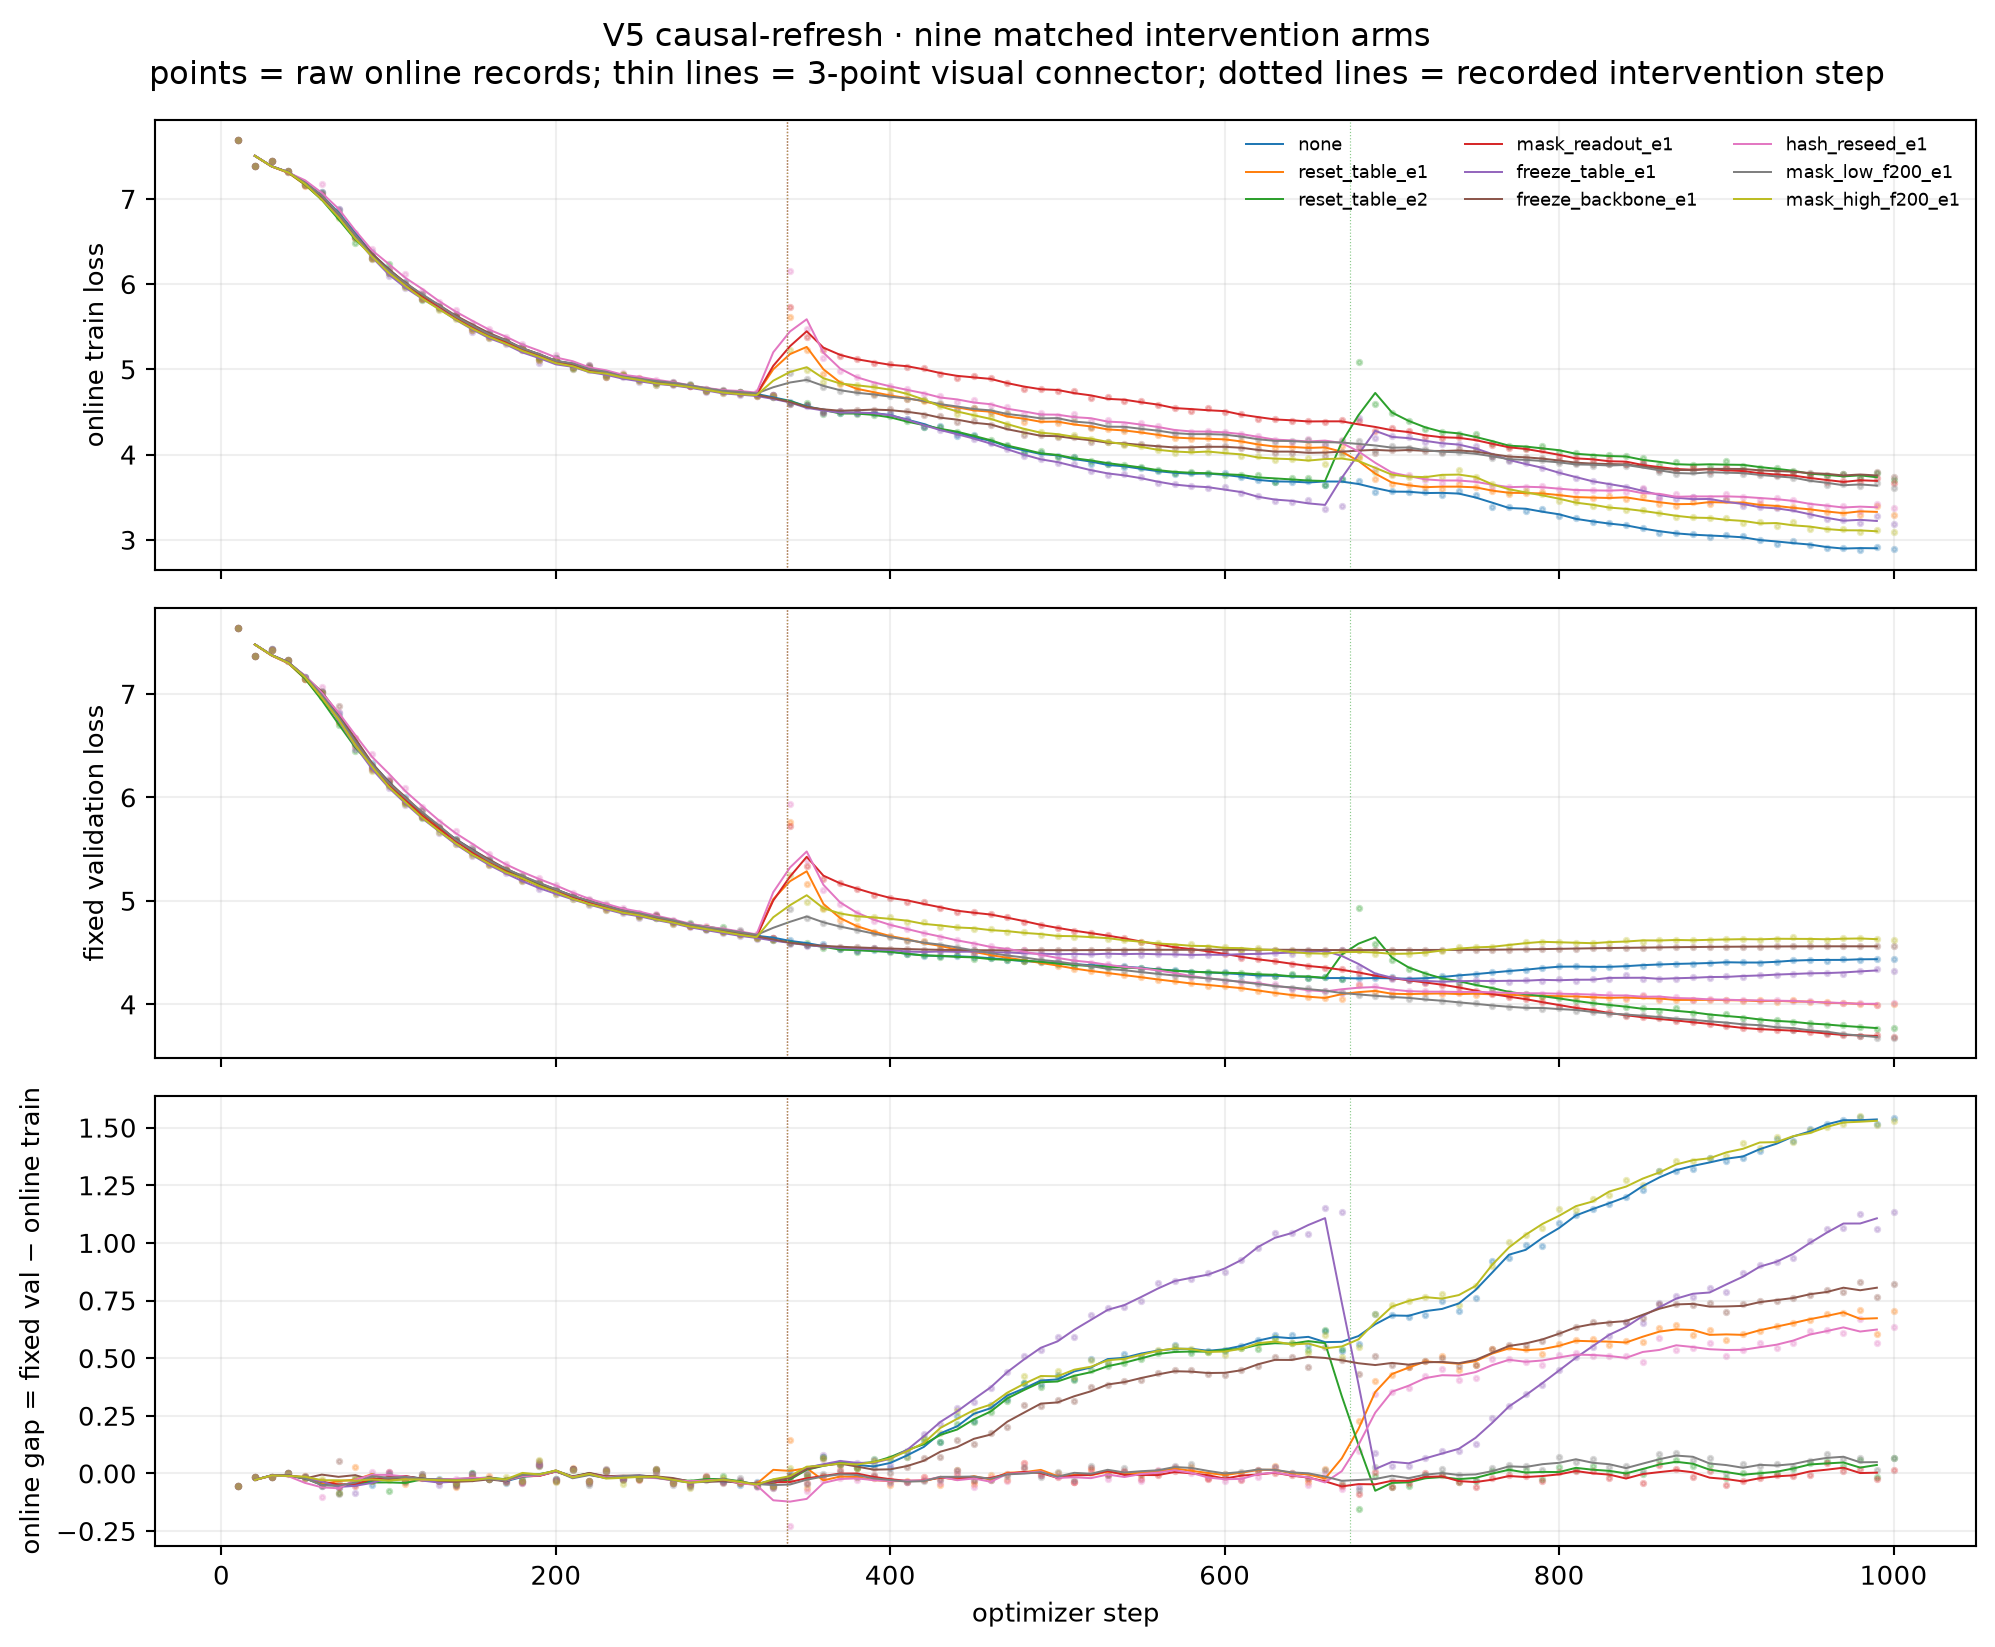
\includegraphics[width=0.94\linewidth]{fig_v5_causal_losses.png}
\caption{Training, validation, and gap trajectories for the component interventions. The hash-reseeding condition changes the context-to-row mapping at each epoch while retaining table weights and optimizer state. Its reported endpoint raw gap is 0.069.}
\label{fig:causal-full}
\end{figure}

\begin{table}[!htbp]
\centering\small
\caption{Intervention summary across comparisons in the current draft, not a list of endpoints for Figure~\ref{fig:causal-full}. Raw gaps and relative reductions have different denominators. Exact run and checkpoint metadata for these source-reported numbers remain to be completed.}
\label{tab:causal}
\begin{tabular}{@{}p{0.18\linewidth}p{0.34\linewidth}p{0.42\linewidth}@{}}
\toprule
Condition & Intervention & Reported observation\\
\midrule
No-gram & Remove the n-gram module & Raw gap 0.233; ordinary train--validation differences remain.\\
N-gram & Input injection; table LR $128\times$ & Raw gap 5.676, with replay-related steps.\\
Low-frequency mask & Mask low-count reads in training and evaluation & $F\leq8$ removes about 72\% of net gap; higher thresholds further reduce it.\\
High-frequency mask & Mask high-count reads & Much smaller change than low-frequency masking in the tested comparison.\\
Hash reseed & Change context-to-row mapping each epoch; retain parameters and optimizer & Raw gap 0.069; substantial suppression of replay accumulation.\\
Freeze table & Stop table updates from epoch 2 & About 94\% of second-pass gap remains; growth returns in epoch 3, at a lower level than the two-pass reference.\\
Freeze backbone & Stop backbone updates from epoch 2 & Slightly smaller second-pass gap; little further growth in epoch 3.\\
\bottomrule
\end{tabular}
\end{table}

\figpending{The source high-frequency scan uses the old strict condition $F>t$. It is preserved as an asset but must be replaced by the intended $F\geq t$ scan before a threshold-matched comparison is presented.}{High-frequency masking: replacement plot pending under the inclusive threshold convention.}

The source analysis reports approximately linear aggregate growth over a 20-pass window, with a slope of 0.664 per pass and $R^2=0.998$. The 20-pass trajectories appear in the right panels of Figure~\ref{fig:staircase}; Figure~\ref{fig:long-replay} retains a separate, earlier 10-pass comparison. Boundary jumps account for approximately 28\% of the accumulated gap in the source analysis, and their share decreases over passes. This motivates a dynamical account that includes within-pass changes, rather than attributing all damage to an instantaneous epoch transition. A finite-window linear fit does not establish unbounded long-run growth.

\begin{figure}[!htbp]
\centering
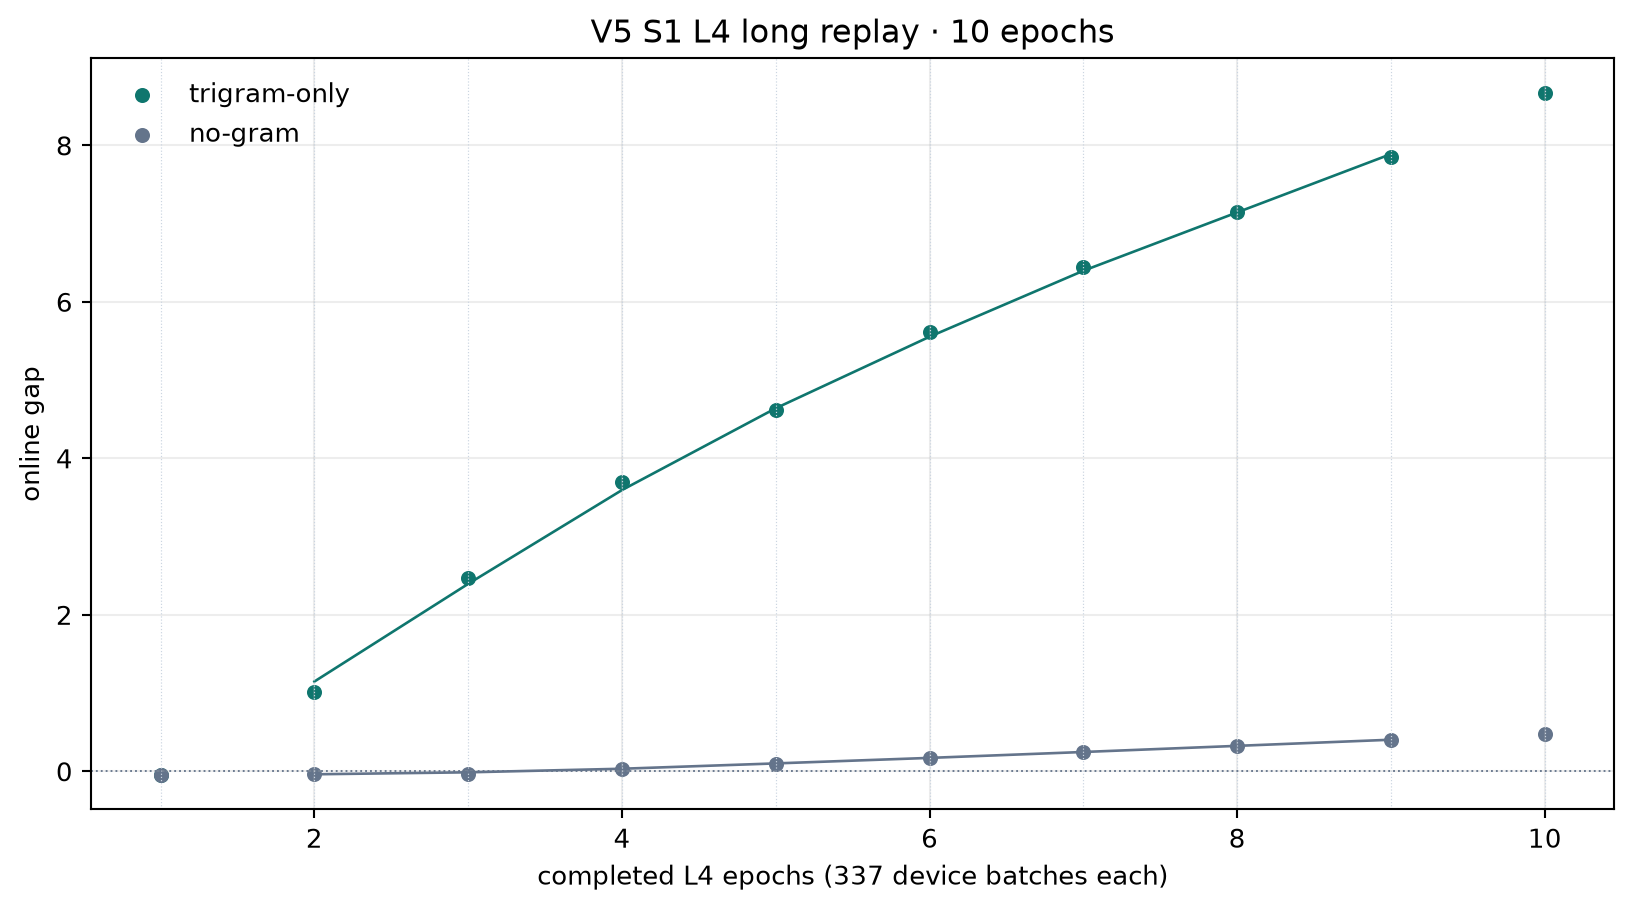
\includegraphics[width=\linewidth]{fig_v5_s1_long_replay.png}
\caption{Archived 10-epoch trigram-only replay comparison with a no-gram control. The Chinese source caption describes 20 epochs, but the embedded image covers ten. The image is retained here with its actual scope; it is not the evidence for the 20-pass fit quoted in the text.}
\label{fig:long-replay}
\end{figure}

A reduced gap must be distinguished from improved validation performance: increasing training loss can shrink the difference without repairing generalization. Likewise, a gap that survives table freezing does not imply that all relevant memory is stored in the table. In the strong-replay comparison recorded in the source, validation loss is approximately 6.95 with n-gram memory and 3.34 without it. Figure~\ref{fig:net-benefit} compares absolute validation changes relative to the no-gram baseline. In this regime, the additional memory does not provide a net generalization benefit.

\begin{figure}[!htbp]
\centering
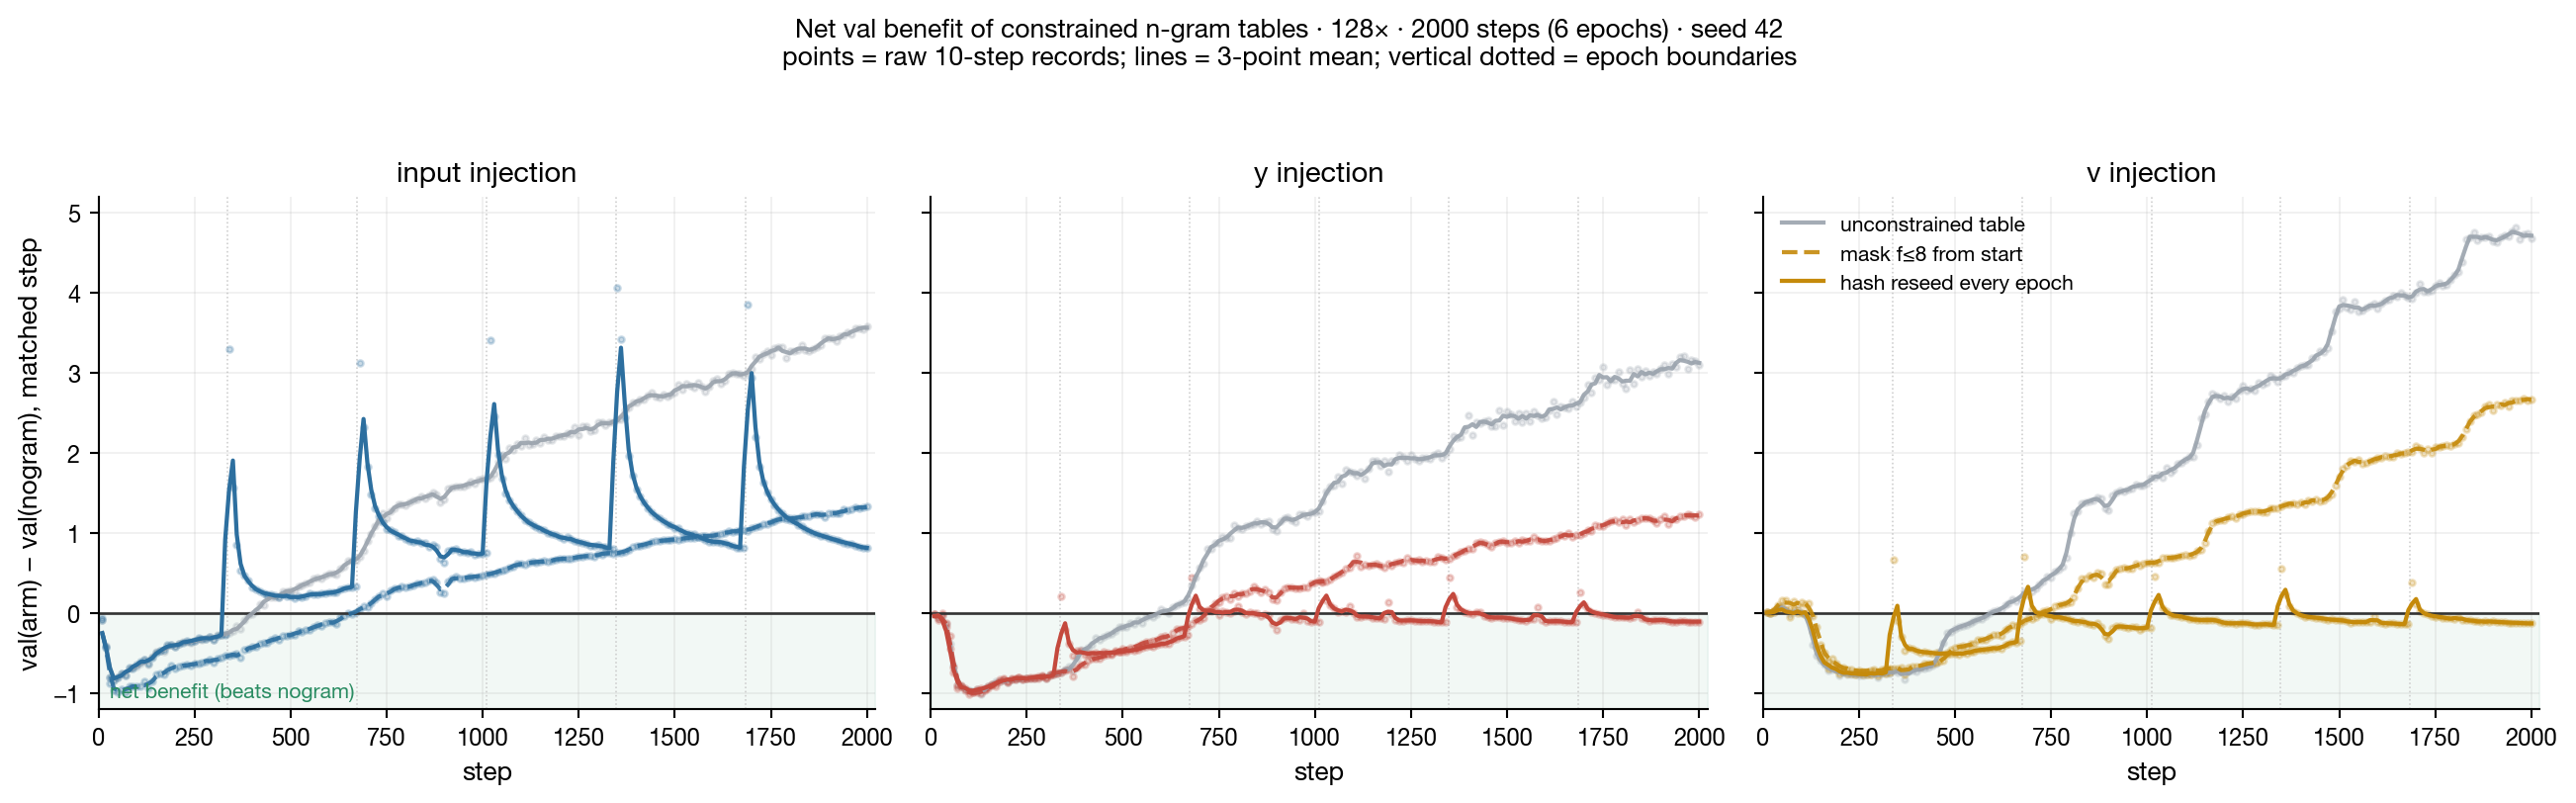
\includegraphics[width=\linewidth]{fig_v5_netval_benefit.png}
\caption{Validation-loss differences relative to the no-gram baseline in the source intervention analysis. These comparisons delimit the benefit of memory in the measured replay regime; they do not establish that n-gram memory should only be used as a short-term cache.}
\label{fig:net-benefit}
\end{figure}

Low-frequency masking and reseeding are mechanism-motivated interventions, but their practical value also depends on preserved training benefits and additional cost. The choice between refreshing memory, retaining it, or protecting selected keys requires evidence under the intended data coverage and training history.

\section{Mathematical Derivations and Model Tests}
\label{app:math}

\subsection{Conditional continuation tails and the novel-continuation rate}
For a context $c_i$ with $F_i=F$, let $y_{i,(r)}$ denote the $r$-th most likely continuation and $p_{i,(r)}$ its true conditional probability. Model the observed continuations $Y_{i,1},\ldots,Y_{i,F}$ as independent draws, with counts $n_{i,(r)}(F)=\#\{k\in\{1,\ldots,F\}:Y_{i,k}=y_{i,(r)}\}$. The novel-continuation rate $f_i(F)$ (the Good--Turing missing mass) and its expectation under this sampling model are
\begin{equation}
f_i(F)=\sum_r p_{i,(r)}
\mathbf{1}\left[n_{i,(r)}(F)=0\right],
\quad
\mathbb{E}[f_i(F)]=\sum_r p_{i,(r)}(1-p_{i,(r)})^F.
\end{equation}

Assume a conditional tail $p_{i,(r)}\sim A_i r^{-s}$ with $s>1$. Using $(1-p_{i,(r)})^F\approx e^{-Fp_{i,(r)}}$ gives
\citep{gnedin2007occupancy}
\begin{equation}
\begin{aligned}
\mathbb{E}[f_i(F)]
&\sim
\int_1^\infty A_i r^{-s}e^{-F A_i r^{-s}}\,\mathrm{d}r\\
&\sim
\frac{A_i^{1/s}}{s}
\Gamma\left(1-\frac{1}{s}\right)
F^{-(1-1/s)}\\
&\propto F^{-\alpha},
\quad
\alpha=1-\frac{1}{s}.
\end{aligned}
\label{eq:occupancy}
\end{equation}

This provides a conditional explanation of the empirical scaling. Finite vocabulary restricts the power law to an intermediate range, correlated observations and context heterogeneity can further change the effective exponent.

\subsection{Crowding-out within a context subspace}
\label{app:crowding-derivation}

Fix a context $c_i$ and call the next-token logits computed from it, $a_v$ for $v$ in the vocabulary, its \emph{context subspace}; the $n$-gram table gives $c_i$ a learned coordinate, so these logits can move without moving those of other contexts (Section~\ref{sec:context-locality}). Partition the vocabulary into the continuations of $c_i$ seen in training ($\mathcal{S}$), those that occur only in validation ($\mathcal{V}$), and the rest. With $p_v=\softmax{a_v}$, one idealized gradient step on a training target $C\in\mathcal{S}$ moves every logit by
\begin{equation}
a_v^{(t+1)}-a_v^{(t)}=-\eta\frac{\partial\ell_C}{\partial a_v}=-\eta\left(p_v^{(t)}-\mathbf{1}[v=C]\right),\qquad \eta>0,
\label{eq:av}
\end{equation}
raising $a_C$ by $\eta(1-p_C)$ and lowering every other logit by $\eta p_v$. For any $u\notin\mathcal{S}$ the odds $z(t)=p_C^{(t)}/p_u^{(t)}$ therefore satisfy
\begin{equation}
z(t+1)=z(t)\exp\!\left[\eta\left(1-p_C^{(t)}+p_u^{(t)}\right)\right]>z(t),
\label{eq:zt}
\end{equation}
and nothing saturates while $p_C<1$. When $\mathcal{S}$ is a single token, the training loss is $-\ln p_C$ and each pass transfers mass from $\mathcal{V}$ and the rest onto $C$; the validation loss on $\mathcal{V}$ rises by the same logit shift that lowers the training loss. Section~\ref{sec:sharpening} identifies $\ln z$, averaged over $\mathcal{V}$, with the depth $D_j$ of Equation~\eqref{eq:gap-decomp}.

\subsection{Position-class decomposition of the excess validation loss}
\label{app:novel-share}

Table~\ref{tab:novel-share} decomposes the both-table model's excess validation loss over the no-gram control (runs \code{s1v5_128_marm_both_ckpt_fixed} and \code{s1v5_128_marm_nogram_ckpt_fixed}, seed 42, step 1000) by whether the true continuation followed its context in the training shard. Contexts are counted at bigram or trigram granularity; \emph{novel} includes positions whose context itself is absent from training.

\begin{table}[!htbp]
\centering\small
\caption{Share of the step-1000 excess validation loss ($1.68$ nats per token, 589{,}248 positions) carried by each position class.}
\label{tab:novel-share}
\begin{tabular}{llrr}
\toprule
context & class & share of positions & share of excess loss \\
\midrule
bigram & novel continuation & 31\% & 73\% \\
bigram & novel or seen with $F\le 31$ & 39\% & 77\% \\
trigram & novel continuation & 66\% & 100\% \\
\bottomrule
\end{tabular}
\end{table}

%\subsection{Data volume, epoch length, and table capacity}
%\label{app:data-volume}

%If the context set is fixed, each $F(i)$ is multiplied by $k$, validation weights remain unchanged, and the per-event damage amplitude is fixed, a missing-mass law with a common exponent gives
%\begin{equation}
% \sum_i w_i A_j c_i[kF(i)]^{-\alpha} =k^{-\alpha}\sum_i w_i A_j c_iF(i)^{-\alpha}.
%\end{equation}
%These assumptions are restrictive. Adding independent data can change the context set, continuation coverage, and the effective frequency distribution. At a fixed step budget, it also changes the number of replays. Fixed-step and fixed-pass comparisons are therefore needed to separate coverage from repeated reinforcement.

%The measured decay is faster than coverage alone: in the dose sweep of Figure~\ref{fig:corpus-size}, the epoch-3 gap falls with corpus size with a local log-log slope of about $0.15$--$0.26$ below $2D_1$ but $0.8$--$0.95$ above it, whereas $k^{-\alpha}$ with $\alpha\in[0.23,0.38]$ predicts a constant slope of at most $0.38$. The missing factor is load suppression. The number of distinct contexts $K(D)$ grows with the corpus while $R$ stays fixed, and an empirical dilution surface built from the single-table bigram table-size sweep (\code{s1v5_128_tbl_bi1_R*_fixed}, seed 42, step 1000) shows a suppression factor $a(K/R)$ that is nearly flat in context frequency and scales approximately as $(K/R)^{-0.59}$ over loads $10$--$1000$; the same exponent accounts for the table-size slope of Figure~\ref{fig:capacity}. Combining the two factors, $\operatorname{gap}(D)\approx A(\text{passes})\cdot a(K(D)/R)\cdot\sum_f \mu_f M(f)$: coverage supplies the $D^{-\alpha}$ part, load suppression steepens the middle range, per-context damage saturation caps the small-$D$ end, and the replay-free residual bounds the large-$D$ end, where the memory-specific component of the gap vanishes. The function $a(\cdot)$ is an empirical factor; its microscopic origin (backbone readout calibration versus row-level traffic competition) remains open.

%Hash collisions may reduce the independence of local memory signals, but they can also mix unrelated contexts; they are one candidate micro-origin of the load factor above, not yet separated from the backbone-readout channel.

%\pending{Complete token-mass-weighted aggregation when the frequency distribution changes, the collision model, and matched data-volume experiments. The epoch-length figure is awaiting replacement. Closing the dose axis additionally requires the distinct-context count $K(D)$ at each dose.}

%\subsection{Further tests of multi-epoch dynamics}

%\pending{Derive the optimizer-dependent margin evolution and align it with measured per-pass damage. Distinguish approximately linear accumulation over a finite window, decreasing increments, and a possible long-run plateau. Specify observations that would falsify the model. The local margin, transfer coefficient, and aggregate gap slope currently serve as constraints, not a closed derivation.}

\subsection{Frequency-scaling fits}
\label{app:gt-fits}

The Good--Turing novel-continuation rate is recomputed from the raw training shard (seed-42 \code{shard_00001.bin}, 49.7M positions, chunked exactly as the data loader chunks it) as $\hat f(F)=N_1(F)/(F\,n(F))$, where $n(F)$ is the number of contexts with exact count $F$ and $N_1(F)$ the number of context--continuation types occurring once among them. Figure~\ref{fig:b_t_MF} shows every positive exact-$F$ layer. Beyond $F\approx10^3$ each layer holds only a handful of contexts (0.1\% of bigram contexts and fewer than 0.01\% of trigram contexts lie there) and the estimates fan out by two orders of magnitude from sampling noise. A fit that weights every layer equally over the full range is dominated by this tail and returns $\alpha=0.45$ (bigram) and $0.43$ (trigram); the version of this figure in an earlier draft, which fitted the per-count total $F\hat f(F)$ the same way, gave $0.34$ and $0.38$. We therefore fit on $F\le10^3$, the window in which the gap is measured and which holds 76\% (bigram) and 97\% (trigram) of training tokens, and weight each context equally, which is the estimator of the per-context mean that Equation~\eqref{eq:gap_j} averages. Under this weighting the tail no longer matters (the fit is unchanged if the window is widened to all $F$), and the exponents are $0.287$ and $0.314$. Weighting by tokens ($F\,n(F)$) instead gives $0.266$ and $0.246$; the spread between the two weightings, about $0.02$ for bigram and $0.07$ for trigram, is the corpus-side uncertainty of the exponent.

\begin{figure}[!htbp]
\centering
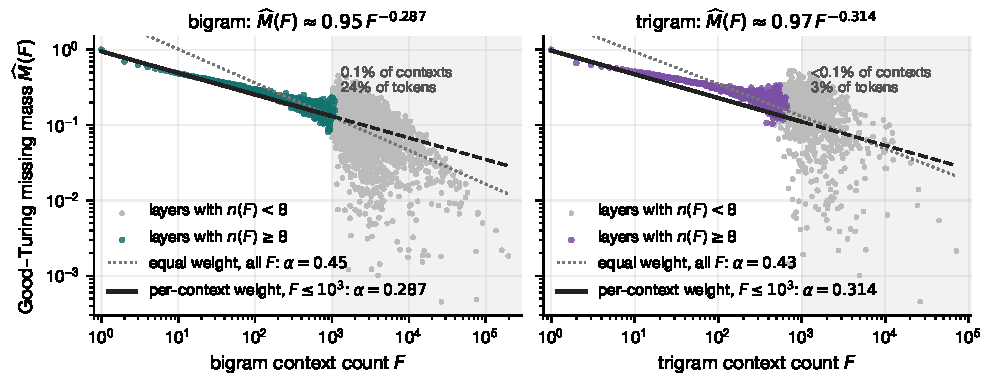
\includegraphics[width=\linewidth]{fig_app_gt_missing_mass.pdf}
\caption{Good--Turing novel-continuation rate $\hat f(F)$ by exact context count for bigram (left) and trigram (right) contexts. Coloured points are layers with at least 8 contexts, grey points sparser layers; the shaded region $F>10^3$ is excluded from the per-context-weighted fit (solid, extrapolated dashed). The dotted line is the equal-weight full-range fit.}
\label{fig:b_t_MF}
\end{figure}

Figure~\ref{fig:gt-kernel} compares the gap with $D\,\hat f(F)$ in the seven geometric frequency bins of the registered gap fit (run \code{s1v5_128_frequency_main}, seed 42, step 1000, fixed train probe and fixed validation loss, bins restricted to at least 32 shared contexts), pooling $\hat f$ over the same bins. With $D$ the geometric mean of $\operatorname{gap}/\hat f$ over the bins, the ratio is constant to within 9\% (bigram) and 18\% (trigram) across 2.5 decades of $F$, and $\log\operatorname{gap}$ correlates with $\log\hat f$ at $0.99$ and $0.98$. The trigram ratio drifts downward with $F$: the gap decays somewhat faster than the novel-continuation rate, so the depth per unit of novel mass, $D$, is not exactly frequency-independent for trigram contexts---rarer contexts are hurt slightly more per novel token, consistent with sharper memorization when fewer distinct continuations were seen. This, together with the 27\% of excess loss that falls on seen continuations of frequent contexts (Table~\ref{tab:novel-share}), is the part of the gap that coverage alone does not account for.

\begin{figure}[!htbp]
\centering
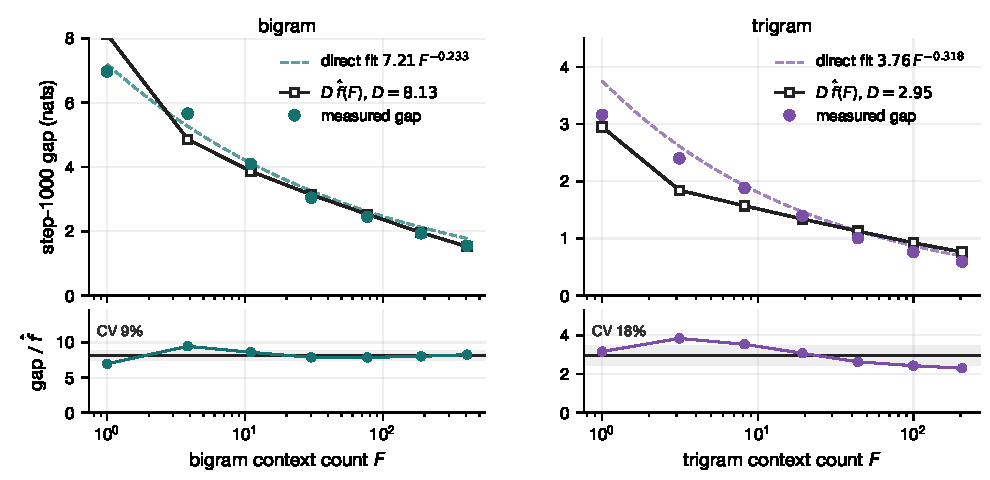
\includegraphics[width=\linewidth]{fig_app_gt_kernel.pdf}
\caption{Step-1000 gap against $D\,\hat f(F)$ in the seven matched frequency bins (top) and the per-bin ratio $\operatorname{gap}/\hat f$ with its mean and $\pm$CV band (bottom); dashed lines are the direct power-law fits of Equation~\eqref{eq:gap-fits}.}
\label{fig:gt-kernel}
\end{figure}

\section{Experiment and Figure Provenance}
\label{app:provenance}

The English draft is based on revision 2633 of the current Chinese manuscript, retrieved on 16 September 2026. The local source snapshot retains the original section text and figure identifiers. Figure assets were downloaded without changing their data. Legacy figure labels that use $f$ for the context count are explained in captions; the manuscript uses $F$ for that count and $f$ for novel-continuation mass.

The new DeepSeek-like comparison is generated directly from archived fixed-probe logs. The associated script and provenance file record run names, endpoint measurements, and file hashes. The earlier full-model run that stopped at step 1913 is not extended to 2000 steps; the figure instead uses a separately completed diagnostic repeat. No new training was performed for this migration.

\pending{Complete the run ID, code revision, data split, seed, checkpoint/pass convention, and plotting source for every inherited main and appendix figure. The current local asset manifest identifies the source document blocks, but is not a substitute for a full experimental reproduction manifest.}

\section{Cross-Architecture Replication and Intervention Protocol}
\label{app:deepseek}

Section~\ref{sec:empirical} summarizes the cross-architecture replication; this appendix gives its protocol. The DeepSeek-like configuration is a smaller 12-layer model whose backbone combines MLA-lite attention, a dense SwiGLU first layer, 11 subsequent mixture-of-experts layers with 16 routed experts, top-2 routing and two shared experts, auxiliary-loss-free load balancing, and four-stream mHC. Engram modules at layers 2 and 6 use bigram and trigram retrieval with multi-head hashing, context-dependent gates, and causal local convolution, i.e.\ multi-layer input over-encoding in the formulation of this paper. It is trained for 2000 updates with seed 42, replaying the fixed shard-1 corpus with a fixed validation probe; the backbone uses AdamW with learning rate $0.0006$ and the tables RMSProp with learning rate $0.0768$, with 100 warmup steps followed by constant learning rates. The fixed training and validation probes are evaluated at the same checkpoint. The table below lists the archived runs used in the figure; names are included for internal traceability and can be moved to the released artifact manifest for submission.
\begin{figure}[!htbp]
\centering
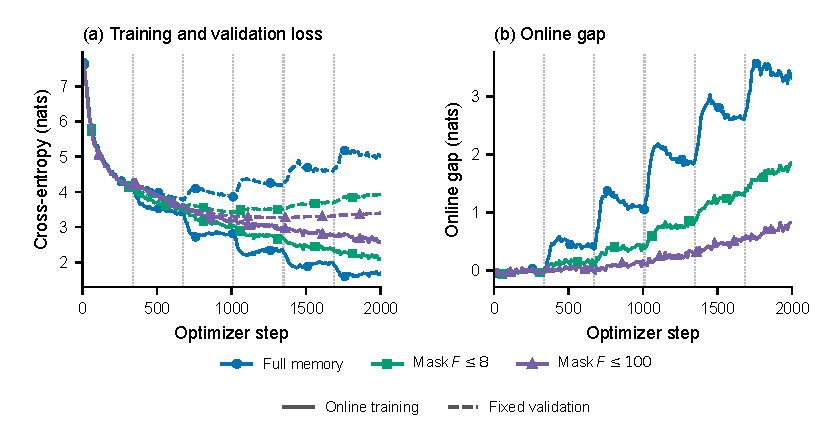
\includegraphics[width=\linewidth]{fig_deepseek_read_masks.pdf}
\caption{Forking and low-frequency retrieval masking in the DeepSeek-like model. (Left) Online training loss (solid) and fixed validation loss (dashed). (Right) Their difference. Colors and markers identify the unmasked model and two masking thresholds. Vertical dotted lines mark replay boundaries; line segments connect raw logged values.}
\label{fig:deepseek}
\end{figure}

\begin{table}[!htbp]
\centering\small
\caption{DeepSeek-like runs used for the fixed-probe comparison. All use seed 42.}
\label{tab:ds-runs}
\begin{tabular}{@{}lp{0.69\linewidth}@{}}
\toprule
Condition & Archived run ID\\
\midrule
Full repeat & \path{dscont_v1_full_fault_s42_2k_fixed}\\
Mask $F\leq8$ & \path{dscont_v1_maskle8_e2_s42_2k_fixed}\\
Mask $F\leq100$ & \path{dscont_v1_maskle100_e2_fault_s42_2k_fixed}\\
All-read mask & \path{dscont_v1_maskall_e0_fault_s42_2k_fixed}\\
\bottomrule
\end{tabular}
\end{table}

The low-frequency conditions suppress retrieved vectors from step 338 onward, according to counts in the original training frequency index. They retain table parameters, optimizer state, and the remaining fusion operations. The completed full-memory and $F\leq100$ runs include additional non-finite diagnostics. These runs have separate training trajectories and were not resumed from one shared pre-intervention checkpoint. Their agreement is therefore a same-seed, configuration-level comparison, not a bitwise-matched checkpoint intervention.

For the all-read mask, the first failure report records an Inf at step 96 on the input boundary of \path{blocks.8.ffn.shared_experts.0.down.0}. The run completed 95 finite updates. It is excluded from endpoint performance comparisons and is not treated as a successful no-memory baseline.

A further mechanism stress test could select contexts with several valid continuations, repeatedly train one, and measure the losses of the others. This asks whether local prediction becomes excessively sharp, rather than merely testing a broad distribution shift. Its feasibility and scope require matched experiments. Neither the current replication nor this proposal establishes a vulnerability in a deployed DeepSeek model.

\pending{Finalize the canonical architecture and data fingerprints, document differences from the minimal setting, and add a stable matched no-memory control. Separate any component-specific claim from the joint-architecture replication.}

\section{Continued-pretraining stress test}
\label{app:sft}

The six runs in Section~\ref{sec:transfer} start from the checkpoint-materialization rerun of the full-pool $20\times$ trigram experiment, with endpoint gap $0.214$ at step 20,220. The original scientific run has the same setting and endpoint gap $0.220$ but does not retain final weights. We restart the backbone AdamW and table RMSProp states and apply a fresh 100-step warmup.

The model is the vanilla 8-layer, 6-head, 768-dimensional NanoGPT with input trigram injection and a clean $2^{20}$-row table. We use seed 42, BF16 forward computation, no compilation, backbone learning rate $6\times10^{-4}$, table learning rate $0.0768$, and fixed validation. Each continued-pretraining source has 333 batches and is run for five epochs (1665 updates); logs are recorded every 10 steps and at the final boundary. The online gap is $G=L_{\mathrm{va}}-L_{\mathrm{tr}}$, where training loss is measured on the current batch before the update and validation loss is measured after the update on fixed batches.

The endpoint measurements are:

\begin{table}[!htbp]
\centering\small
\caption{Endpoint measurements for continued language-model pretraining from the low-gap checkpoint. All values are nats, seed 42, step 1665. The table-trainable and table-frozen runs differ only in whether the trigram lookup table receives gradients.}
\label{tab:sft-results}
\begin{tabular}{llrrr}
\toprule
Source & Table & Train & Validation & Gap\\
\midrule
ID & Trainable & 1.913 & 4.376 & 2.463\\
ID & Frozen & 3.030 & 3.372 & 0.341\\
Magicoder & Trainable & 0.740 & 1.752 & 1.012\\
Magicoder & Frozen & 1.342 & 1.555 & 0.212\\
OpenR1 & Trainable & 0.754 & 1.480 & 0.726\\
OpenR1 & Frozen & 1.226 & 1.324 & 0.098\\
\bottomrule
\end{tabular}
\end{table}

The corresponding dense logs and figures are archived with run IDs \path{sft_*_e5_freq10_{trainable,frozen}_s42}. These are single-seed continued-pretraining measurements, not response-only instruction-SFT results.

\paragraph{Static RLVR-like proxy.}
We additionally ran two continued-pretraining runs on \path{allenai/RLVR-MATH} from the Tulu 3 release~\citep{lambert2024tulu3} (revision \path{bd2a93551b503a395fadd1a740d957559cfe6f3c}), which contains the 7,500 MATH training problems formatted for RLVR. The prompts carry fixed 4-shot exemplar prefixes that are byte-identical across examples, and the \path{ground_truth} field is the reference final answer. The original parquet SHA256 is \path{2fb8483bf7a4ae9821bee1e715490fb8de5b59f0d2b58bd4de78cc75094d9422}. Messages were retained verbatim and the \path{ground_truth} was appended once after an ``Answer:'' marker. The first 95\% and last 5\% of source examples (in original row order) were used as disjoint train and validation pools, then cycled to 333 train batches and 4 validation batches.

The shared setting matches the six runs above: seed 42, 1665 updates, five replay epochs, fresh optimizer state and 100-step warmup, input trigram-only clean $2^{20}$-row table, and fixed validation. In the frozen arm only the table is fixed; the backbone remains trainable. Endpoint measurements are:
\begin{table}[!htbp]
\centering\small
\caption{Static RLVR-like verifier-selected continued-pretraining endpoints. All values are nats at step 1665, seed 42.}
\label{tab:rlvr-results}
\begin{tabular}{llrrr}
\toprule
Source & Table & Train & Validation & Gap\\
\midrule
RLVR-MATH & Trainable & 0.009 & 0.621 & 0.612\\
RLVR-MATH & Frozen & 0.020 & 0.522 & 0.502\\
\bottomrule
\end{tabular}
\end{table}

The run IDs and dense logs are archived under \path{rlvr_static_proxy_20260921}. This is a static verifier-selected proxy, not on-policy reinforcement learning.
